\documentclass[../ala_hataile.tex]{subfiles}
\begin{document}
	\clearpage
		
\includepdf[pages=16-17, pagecommand={}]{sisasivut_19062018.pdf}
\twocolumn[\section{Maantiede tieteenalana}]
Maantieteellä on ollut aina merkitystä
ihmisille. Niin kauan, kun maapallolla
on asunut ihmisiä, on alueiden
ja ilmiöiden sijainnit koettu tärkeäksi.
Vanhin Euroopasta löydetty kartta
on turkkilainen kalliopiirros, joka sijoittuu
vuoteen 6000~eaa. Tieteenalanakin
maantieteellä on pitkät perinteet; maapalloa
on tieteellisesti tutkittu aina antiikin
ajoista saakka.

\begin{figure*}[!b]
	
\includegraphics[width=\textwidth]{isosali.png}
\end{figure*}

Maantiede ei rajoitu kuitenkaan vain
karttoihin ja sijainteihin. Maantiede
tutkii maan pinnalla tietyllä alueella
tapahtuvia ihmisen ja luonnon välisiä
vuorovaikutuksia. Maantieteilijöitä
kiehtovat maan pinnalla esiintyvä alueellinen
erilaistuminen ja sen taustalla
olevat prosessit. Ihmisen ja luonnon
sekä ympäristön ja yhteiskunnan välinen
suhde on olennaisessa asemassa.
Maantieteelliset ilmiöt voidaan myös
sitoa jonkinlaiseen mittakaavaan: ne
voivat olla niin paikallisia kuin globaalejakin.
Maantiede on tieteenä laaja-alainen.
Niin luontoihmiselle, kulttuureista
ja taloudesta kiinnostuneille sekä
tietokoneella työskentelystä innostuneelle
löytyy oma maantieteen ala.

\subsection*{Maantiede Helsingin yliopistossa}
Helsingin yliopiston maantieteen koulutusohjelmassa on
kaikille tiedonhaluisille useita vaihtoehtoja. 
Pääasiallisia erikoistumislinjoja ovat geoinformatiikka, 
luonnonmaantiede, kaupunkimaantiede, 
suunnittelumaantiede ja ihmismaantiede. 
Kaupunki-, suunnittelu- ja ihmismaantieteessä 
tarkastellaan ihmisten suhdetta
ympäristöön ja siinä tapahtuvia muutoksia.
Näitä muutoksia tutkitaan alueiden
tai aluejärjestelmien avulla paneutuen etenkin
alueelliseen erilaistumiseen ja siihen vaikuttaviin tekijöihin.
Myös aluekehitys ja alueellinen kehittäminen ovat  
olennaisia koulutuksen teemoja.
Maantieteen tehtävänä on myös tulkita 
luonnon ja ihmisen muodostamien
alueellisten ja paikallisten järjestelmien
syntyä ja kehitystä. Geoinformatiikassa
keskeistä on alueellisen,
paikkaan sidotun tiedon tuottaminen,
analysointi ja visualisointi. Luonnonmaantieteessä
keskitytään puolestaan luonnonjärjestelmiin, 
kuten ilmaston ja hydrologian vaikutuksiin.

\subsection*{Opintojen kulku}
Fuksit opiskelevat 
koko vuoden yhteisiä perus- ja aineopintoja, sekä käyvät muutamia yliopiston käytäntöihin ohjaavia kursseja. 
Toisena opiskeluvuotena on tavoitteena
suorittaa menetelmätieteitä, vapaasti valittavia opintoja ja kieliopinnot.

Maantieteilijällä on monia vaihtoehtoja vapaasti valittaviin opintoihin.
Opintoja voi
maantieteeseen yhdistää lähes mitä
vain, onhan maantieteellä useita
erikoistumislinjojakin. Kannattavaa
on tietenkin valita aine, joka tukee
omia maantieteen opintoja. Suosittuja
kokonaisuuksia ovat olleet Aallon
yhdyskunta- ja kaupunkisuunnittelu,
ympäristötieteet, biologia ja
pedagogiset opinnot sekä erilaiset
valtiotieteellisen tiedekunnan kurssit.
Maantieteen fukseille järjestetään joka
kevät erityinen opintokokonaisuusinfo helpottamaan
valinnan vaikeutta. Lisätietoa
opintokokonaisuusinfosta löytyy MaO~ry:n kotisivuilta
(\url{https://blogs.helsinki.fi/maantieteenopiskelijat-ry/}).

Kolmantena opiskeluvuotena
suoritetaan loput aineopinnot, jatketaan valinnaisia opintoja sekä mahdollisesti
täydennetään opintoja niin, että kandidaatin
tutkintoon tarvittavat 180~op
saadaan kasaan.

\subsection*{Maantiede sivutieteenalana}
Koska maantiede on varsin laaja-alainen
tiede, se käy sivu\-tieteen\-alaksi moniin
muihin koulutusohjelmiin. Maantieteen opiskelija oppii niin luonnontieteellistä
ajattelua, yhteiskunnallisia
teemoja, tietokonepainotteista geoinformatiikkaa
kuin maantieteen uusimpia
tuulia. Maantieteen perusopinnot (25~op) on kaikille yliopistolaisille vapaasti valittava lyhyt opintokokonaisuus. Mikäli
maantieteen opintoja haluaa suorittaa
laajemmin, on haettava matemaattis-luonnontieteelliseltä
tiedekunnalta suoritusoikeutta
aineopintoihin (35~op).
Suoritusoikeuksia maantieteen aineopintoihin
myönnetään kuitenkin
oppimistiloista johtuen vain rajoitetusti.
Haku on vuosittain huhtikuussa
ja opinto-oikeuden saamisen perusteena
on perusopintokokonaisuuden
suoritustaso.

Maantiedettä opiskellaan monissa
erilaisissa muodoissa. Osa perusopinnoista
käydään laajoina massaluentoina.
Luentojen lisäksi opetusmuotoihin
kuuluvat harjoitustyökurssit, kirjatentit,
verkkokurssit, kenttäkurssit sekä seminaarit.
Tenttien lisäksi kursseilla on
sekä kirjallisia että suullisia töitä.


\subsection*{Tuleeko kaikista opettajia?}
Maantieteilijöiden työllistymis\-näkymät
ovat laaja\-pohjaisen koulutuksen
vuoksi erittäin hyvät. Opettaja ja
tutkija eivät suinkaan ole maan\-tieteilijöiden
ainoat työllistymis\-vaihtoehdot.
Yliopisto-opetus tähtää siihen, että
maantieteen alalta valmistuvat ovat
maantieteellisen osaamisen asiantuntijoita.
Työelämässä voidaankin sijoittua
hyvin erilaisiin asian\-tuntija-, hallinto-,
yritys\-toiminta-, suunnittelu-, opetus-,
tutkimus- ja johtamis\-tehtäviin.

Maantieteen opiskelijoiden erikoistumis\-alat
määrittävät pitkälti millaisiin
työtehtäviin valmistutaan. Suuria työllistäjiä
ovat esimerkiksi opetus\-sektorin
lisäksi julkis\-hallinnon suunnitteluja
projektitehtävät, valtion sektori\-tutkimus\-laitokset
sekä myös yrityssektori.
Maantieteilijänä on myös helppo
hakeutua kansain\-välisiin tehtäviin.
Työ\-elämä\-kurssilla tutustutaan haastattelujen
ja työpaikkakäyntien avulla
jo valmistuneiden työpaikkoihin ja "-kokemuksiin. Maantieteen Opiskelijat~ry pyrkii järjestämään monipuolisia yritys\-vierailuja,
jotta maantieteen opiskelijat
pääsevät kartoittamaan konkreettisesti
työllistymis\-vaihtoehtoja.

\twocolumn[\section{Maantieteen kursseja}]
\subsection*{Perusopinnot}
\subsubsection*{Maantiede tieteenalana (5~op)}
Kurssilla useat professorit, opettajat
ja tutkijat käytävät kertomassa omista 
tutkimuksistaan ja avaavat niiden
aihepiiriä laajemmin. Kurssi antaa 
kattavan kuvan maantieteen aihepiireistä,
sekä osastolla tehtävästä tutkimuksesta.

\subsubsection*{Luonnonjärjestelmät maantieteessä (5~op)}
Kurssilla perehdytään luonnonmaantieteeseen
keskeisten osa-alueiden kautta. Kurssilla 
opiskellaan geomorfologiaa, hydrogeografiaa, 
klimatologiaa, biogeografiaa ja käydään läpi 
keskeisiä luonnonmaantieteen
teorioita ja käsitteitä. Kurssilla tutustutaan 
aiheeseen myös kirjallisuuden avulla.

\subsubsection*{Yhteiskunnat ja kaupungit maantieteessä (5~op)}
Kurssilla tutustutaan yhteiskunnan ja kaupunkien
kehitykseen ja suunnitteluun maantieteellisestä
näkökulmasta, sekä avataan aihepiiriin liittyviä
ajankohtaisia teemoja. 

\subsubsection*{Johdatus geoinformatiikkaan maantieteessä (5~op)}
Kurssilla tutustutaan geoinformatiikan perusteisiin 
paikkatiedon perusominaisuuksiin, historiaan ja päätehtäviin paneutuen.
Kurssilla syvennetään myös ymmärrystä projektioista, koordinaateista
ja sijaintitiedoista, sekä opetellaan paikkatiedon tuottamisen
menetelmiä ja tutustutaan aineistolähteisiin.

\subsubsection*{Globaalit tutkimuskysymykset maantieteessä (5~op)}
Kurssilla perehdytään globaaleihin kysymyksiin ja 
vuorovaikutussuhteisiin. Kurssilla käy monia eri 
luennoitsijoita kertomassa oman tutkimusaiheensa
globaaleista kysymyksistä. Kurssilla perehdytään myös 
globaaleihin riskeihin ja riskien eri aluetasoihin.

\subsection*{Aineopintokursseja}
\subsection*{Tiedon esittäminen maantieteessä (5~op)}
Harjoitustyökurssilla perehdytään
maantieteellisen tiedon hankintaan
ja analyysiin. Muun muassa erilaiset teemakartat, kartoilta
mittaaminen ja tilastot tulevat tutuiksi.
Kurssilla tutustutaan myös kartografiaan
karttojen tulkitsemisen ja omien
karttojen tuottamisen kautta. Lisäksi 
kurssilla harjoitellaan maantieteellisen 
raportin tekemistä.

\subsection*{Geoinformatiikan menetelmät~I (5~op)}
Kurssilla tutustutaan paikkatietoaineistoihin
sekä yksinkertaisiin paikkatietoanalyyseihin.
Opetus ja kurssikerrat
kuluvat tietokoneen äärellä. 
Opiskelijat pääsevät itse hyödyntämään 
paikkatietoaineistoja ja analyysejä, sekä tekemään
mielenkiintoisia karttoja ja julkaisemaan niitä
kurssiblogeissaan.

\begin{figure}[h]
	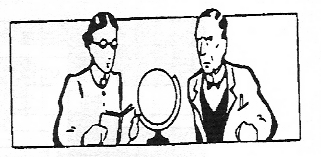
\includegraphics[width=\columnwidth]{karttapallo.png}
\end{figure}
\subsection*{Maantieteen menetelmät (5~op)}
Kurssilla käydään läpi maantieteellisissä
tutkimuksissa käytettäviä menetelmiä luentojen
ja harjoitusten avulla. Kurssilla perehdytään sekä 
laadullisiin että määrällisiin menetelmiin. Lisäksi
jokainen opiskelija pääsee tekemään oman 
geomorfologisen karttatulkinnan.

\subsection*{Maantieteen projektiharjoituskurssi (5~op)}
Kurssilla perehdytään tutkimusprojektin toteuttamiseen
ja sovelletaan opittuja tutkimusmenetelmiä käytäntöön.
Kurssilla opiskelijat työskentelevät kurssilla 
määriteltävän projektityön parissa.
\subsection*{Maantieteen kenttäkurssi (5~op)}
Maantieteilijät lähtevät keväällä Lammille
kenttäkurssille soveltamaan opittuja
taitojaan. Lammilla puuhastellaan
mm.\,hydrologian, korkeuden sekä ilmaston
mittaamismenetelmien ja taajamatutkimuksen
parissa. 

\subsection*{Ihmismaantieteen ja luonnonmaantieteen kirjatentit (5+5~op)}
Kirjatenttien avulla syvennytään 
maantieteen keskeisiin teemoihin
kirjallisuuden avulla. Kirjoissa käsitellään
kattavasti maantieteen kannalta oleellisia
ilmiöitä, teorioita ja käsitteitä, joiden tarkoituksena 
on syventää osaamista eri osa-alueista.

\vspace{0.5cm}\noindent\textsc{Niklas Aalto-Setälä}\\\textsc{Tanja Palomäki}
\end{document}